\appendix
\addcontentsline{toc}{part}{ХАВСРАЛТ}

% Хавсралтын нэр. Хавсралт гэдэг үг агуулахгүй
\chapter{Жишээнүүд}
\begin{figure}
	\centering
	
\includegraphics[scale=2]{src/pictures/zurag1.png}
	\caption{Жишээ-1}
\end{figure}
\begin{figure}
	\centering
	
\includegraphics[scale=2]{src/pictures/zurag2.png}
	\caption{Жишээ-2}
\end{figure}
\begin{figure}
	\centering
	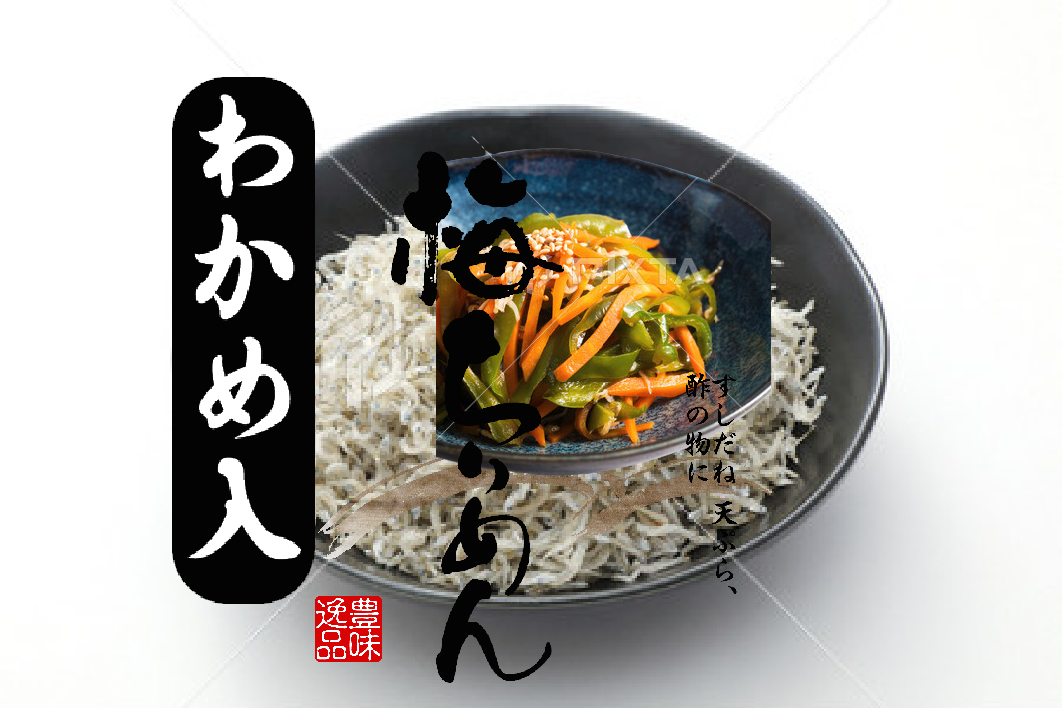
\includegraphics[scale=2]{src/pictures/zurag3.png}
	\caption{Жишээ-3}
\end{figure}

% Хавсралтын нэр. Хавсралт гэдэг үг агуулахгүй
\chapter{Кодын хэрэгжүүлэлт}
\section{Python}
\subsection{Гол script}
\lstinputlisting[language=Python, caption=Text-ээс PNG зураг үүсгэдэг script]{src/code/script.py}
\subsection{Business logic script}
\lstinputlisting[language=Python, caption=Combination үүсгэх бизнес логик код]{src/code/combination.py}
\lstinputlisting[language=Python, caption=Датабазруу КРУД хийх]{src/code/crud.py}